\pagebreak
\subsubsection{divide \& conquer-Ansatz für Präfixsummen}
Als nächstes betrachten wir einen divide \& conquer-Ansatz für die Lösung der Präfixsummen.
\begin{algorithm}[h!]
\caption{Parallele Berechnung der Präfixsummen mit dem divide \& conquer-Ansatz.}
\begin{algorithmic}
\STATE {\bf{function praef }}$(a_1, \dots, a_n)$
\IF {$n=1$} 
\STATE $s_1:=a_1$;
\ELSE
\STATE $s_1 \dots s_{\lfloor\frac{n}{2}\rfloor}:=$\algspawn{\bf{praef}}$(a_1 \dots a_{\lfloor\frac{n}{2}\rfloor})$;
\STATE $s_{\lfloor\frac{n}{2}\rfloor+1} \dots s_{n}:=$\algspawn{\bf{praef}}$(a_{\lfloor\frac{n}{2}\rfloor +1} \dots a_{n})$;
\ENDIF
\FOR{$i:=\lfloor\frac{n}{2}\rfloor+1$ \algto $n$ \algpar}
\STATE $s_i:=s_i + s_{\lfloor\frac{n}{2}\rfloor}$;
\ENDFOR
\end{algorithmic}
\end{algorithm}

\noindent Wie oben bereits erw\"{a}hnt, erzeugt der Befehl \algspawn einen eigenen Thread für den nachfolgenden Befehl.

\noindent{\bf{parallele Laufzeit}}:
\begin{eqnarray*}
T(1) & = & c_1 \\
T(n) & = & T\left(\left\lceil\frac{n}{2}\right\rceil\right)+c_2 \\
\Rightarrow T(n) & = & O(\log n)
\end{eqnarray*} für die Konstanten $c_1$ und $c_2$.\\
Der erste Summand hat keinen Faktor $2$, da beide Funktionen rekursiv ausgeführt werden.
Der zweite Summand $c_2$ kommt von der for-Schleife.
\\\\{\bf{Anzahl der Prozessoren }}:\\
Für Probleme der Größe $1$ benötigt man $1$ Prozessor, f\"{u}r Probleme der Gr\"{o}\ss{}e $n$ ist es 
m\"{o}glich, mit $n$ Prozessoren auszukommen.

\noindent{\bf{Beweis}}(Induktion über $n$):\\
I.A.: $n = 1 \checkmark$
\\I.V.: Die Aussage ist für Zahlen $< n$ richtig.
\\I.S.: Betrachte den else-Fall der if-Abfrage. Der erste rekursive Aufruf be\-n\"{o}\-tigt nach I.V. 
$\lfloor\frac{n}{2}\rfloor$ Prozessoren, der zweite $\lceil\frac{n}{2}\rceil$. In der Summe werden
also $n$ Prozessoren verwendet. Die for-Schleife ben\"{o}tigt sogar nur $\lceil\frac{n}{2}\rceil$
Prozessoren. 
\\
\\
\\\\{\bf{Bemerkungen:}}
\begin{itemize}
 \item Das Zeit-Prozessoranzahl-Produkt ist beim sequentiellen Algorithmus mit $O=(n)$ besser als 
beim parallelen mit $\theta(n\log n)$, es ist aber möglich, eine Laufzeit von $O(\log n)$ mit 
$O(\frac{n}{\log n})$ Prozessoren zu erhalten.
 \item In der for-Schleife lesen $\frac{n}{2}$ Prozessoren den Wert $s_{\lfloor\frac{n}{2}\rfloor}$
gleichzeitig. Dieses concurrent read kann in Wirklichkeit nicht in $O(1)$ realisiert werden.
Es ergibt sich also die Frage, ob man dies f\"{u}r theoretische Betrachtungen trotzdem erlauben soll.
 \item Der Algorithmus funktioniert nicht nur für die $+$-Operation, sondern auch für beliebige andere assoziative (zweistellige) Operationen.
 \item Dies ist eine wichtige Technik beim parallelen Algorithmen.
\end{itemize}

\subsection{Addierer}
Als drittes und letztes Beispiel wollen wir einen 
Schaltkreis zum Addieren von zwei Binärzahlen mit $n$ Stellen $a_{n-1}, \dots, a_0$ und 
$b_{n-1}, \dots, b_0$ mit $a_i,b_i \in \{0,1\}, i=0, \dots, n-1$ betrachten.
\\\\{\bf{Schaltkreis}}(Schaltkreismodell):
\\Wir betrachten Schaltkreise, die aus folgenden Bausteinen bestehen:
\begin{figure}[h!]
\centering
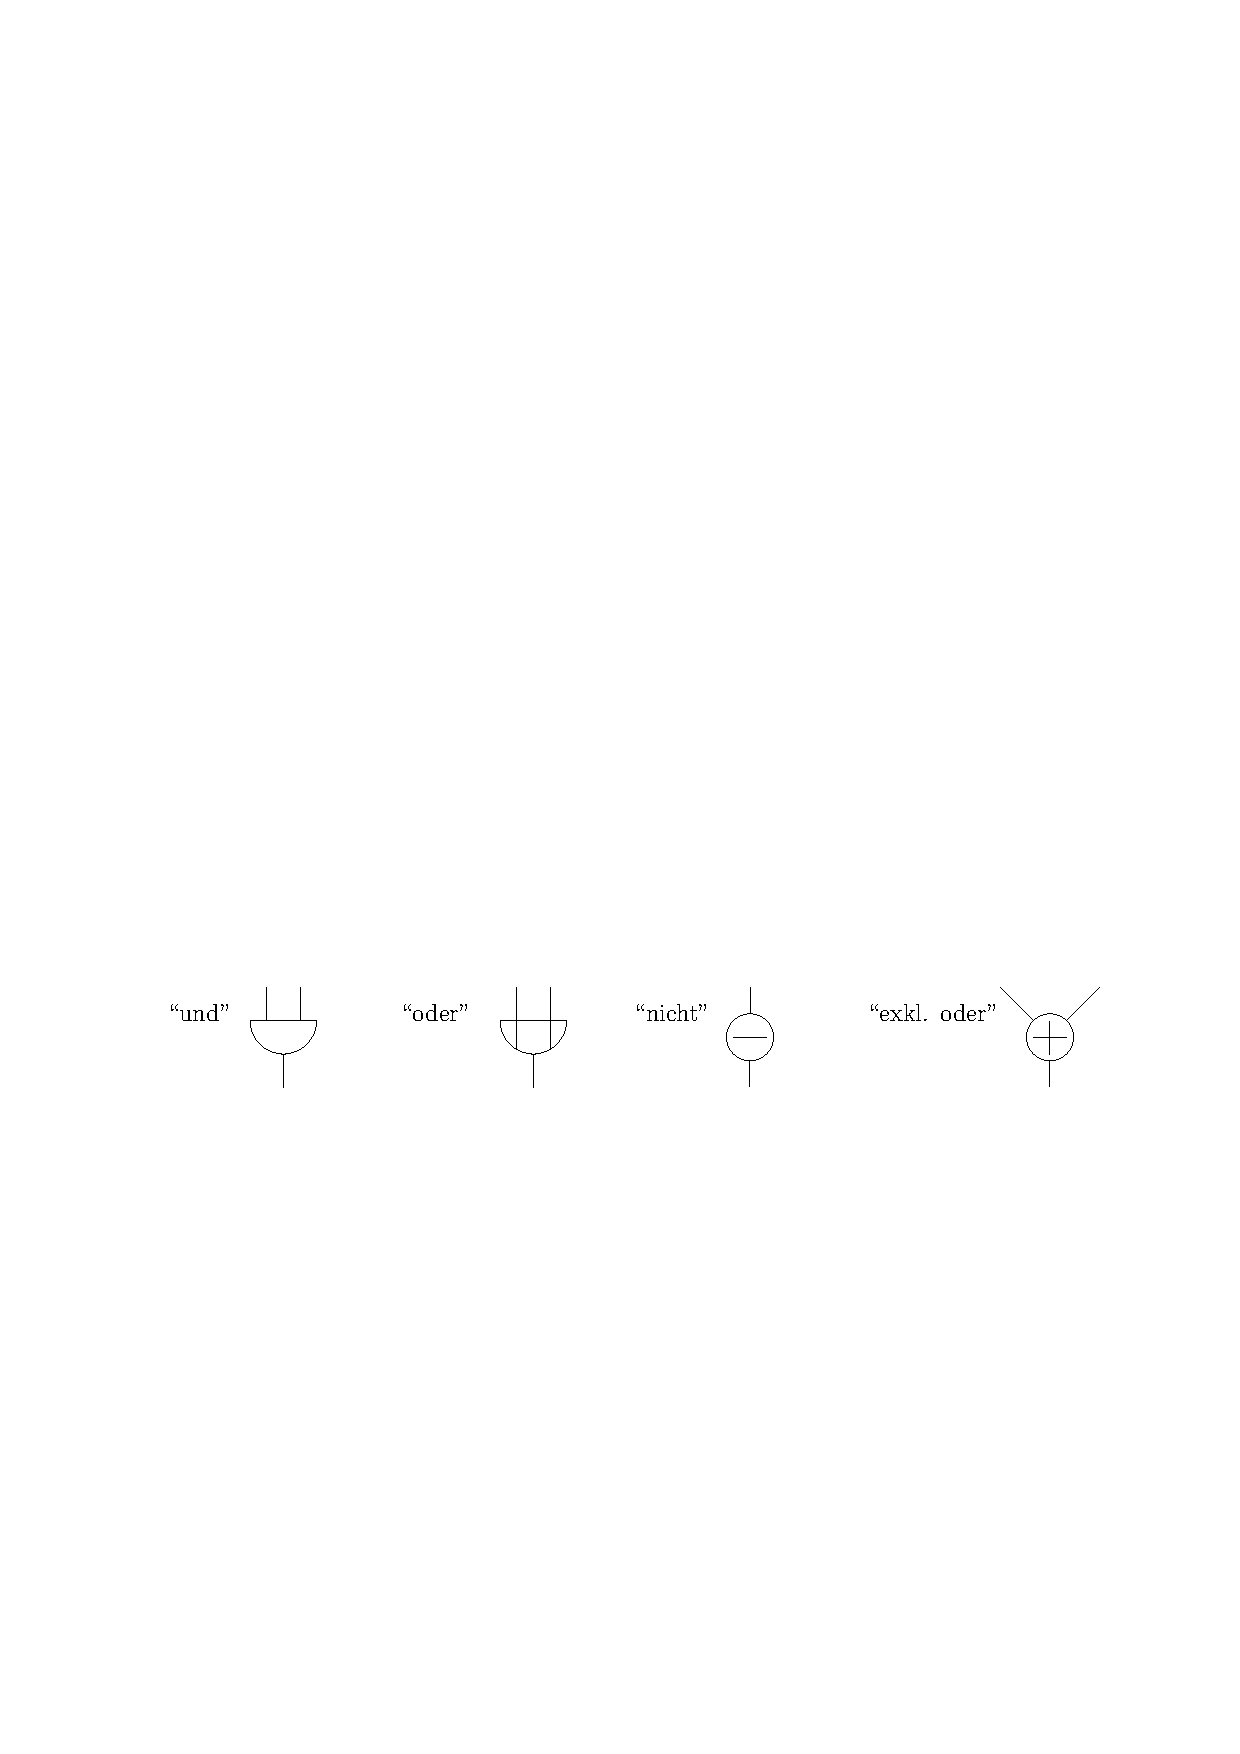
\includegraphics[scale=0.8]{bilder/Bausteine.pdf}
\caption{Grundbausteine von Schaltkreisen.}
\end{figure}
\\\\
% {\bf{Beispiel - Volladdierer:}}
Aus diesen Grundbausteinen l\"{a}sst sich ein Volladdierer zusammensetzen, 
den wir symbolisch wie folgt darstellen:
\begin{figure}[h]
\centering
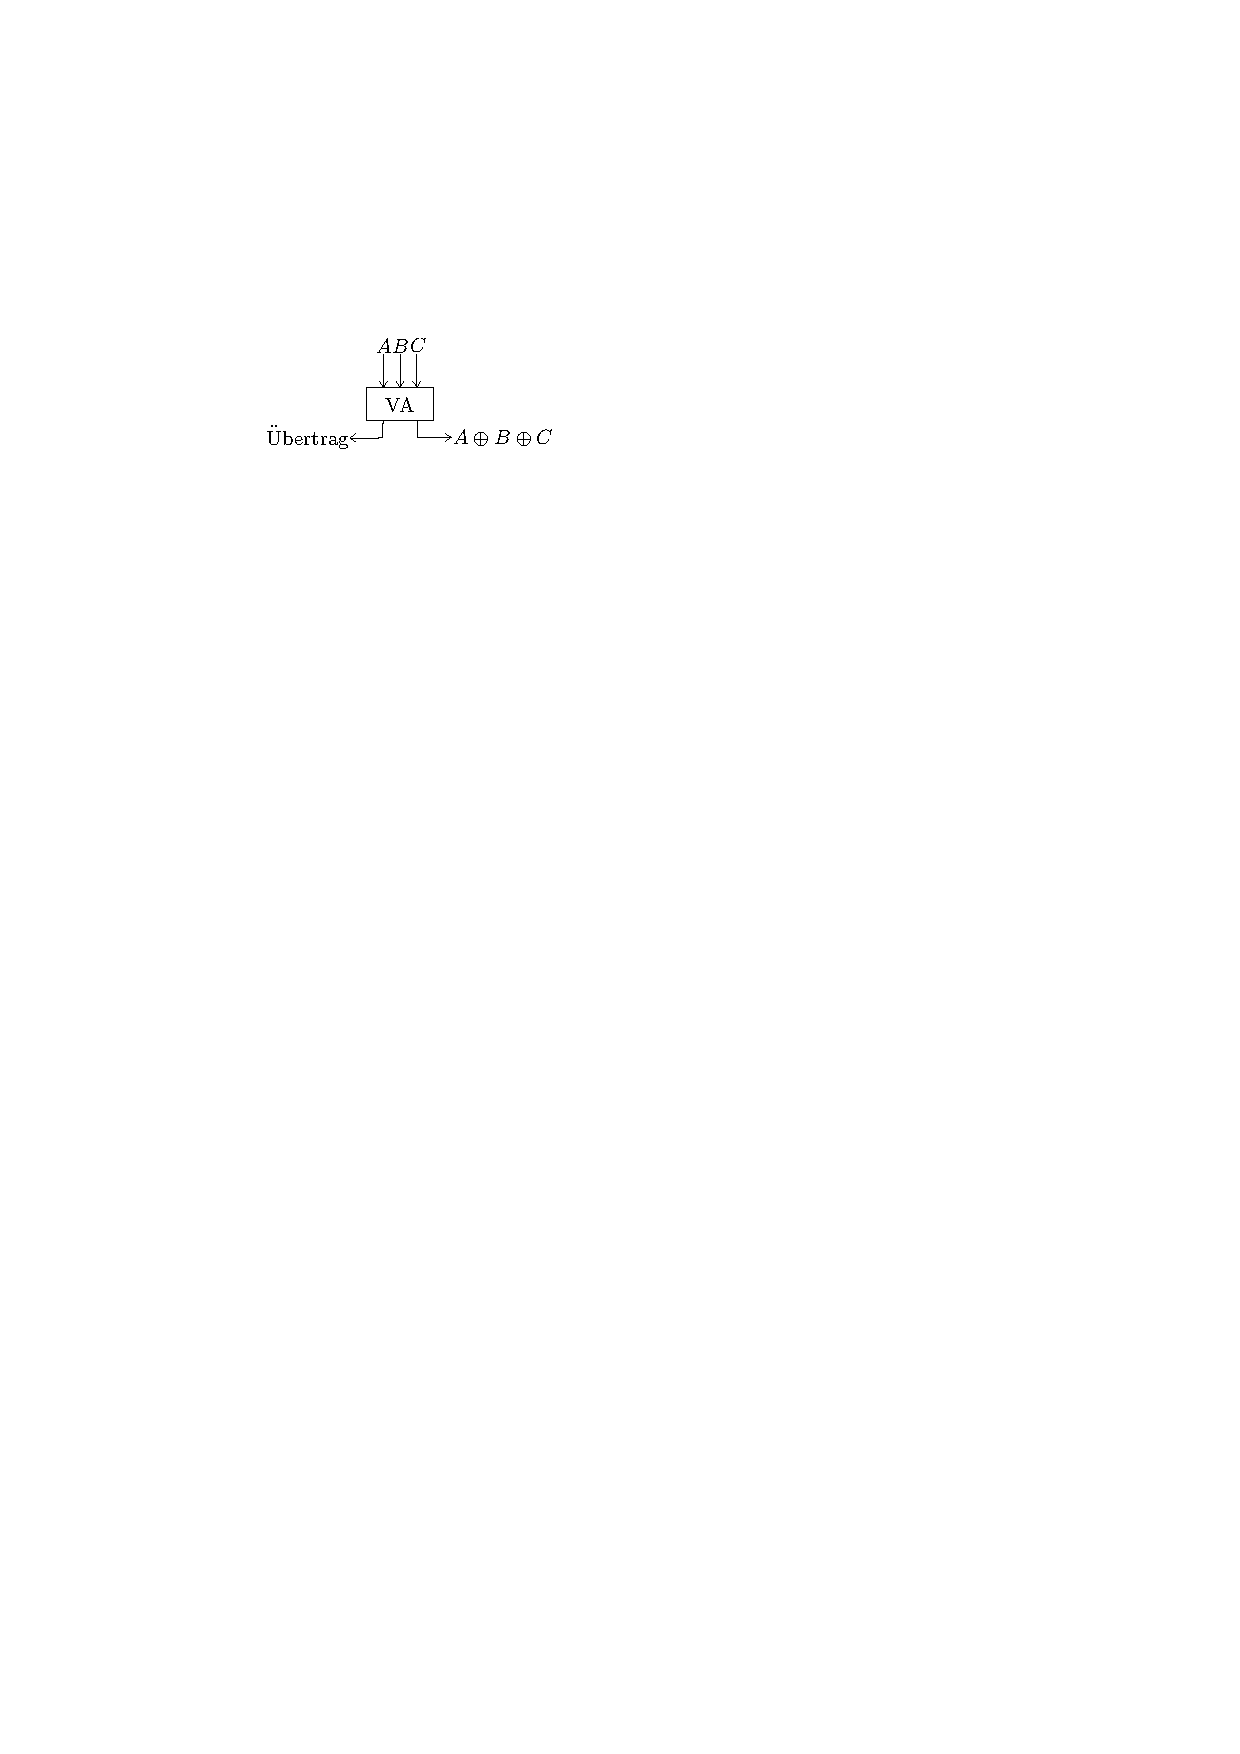
\includegraphics[scale=0.8]{bilder/Volladdierer.pdf}
\caption{Symbolische Schreibweise eines Volladdierers.}
\end{figure}

\noindent Der Volladdierer kann aus den Gattern beispielsweise durch folgenden 
Schaltplan realisiert werden: 
\\
\begin{figure}[h]
\centering
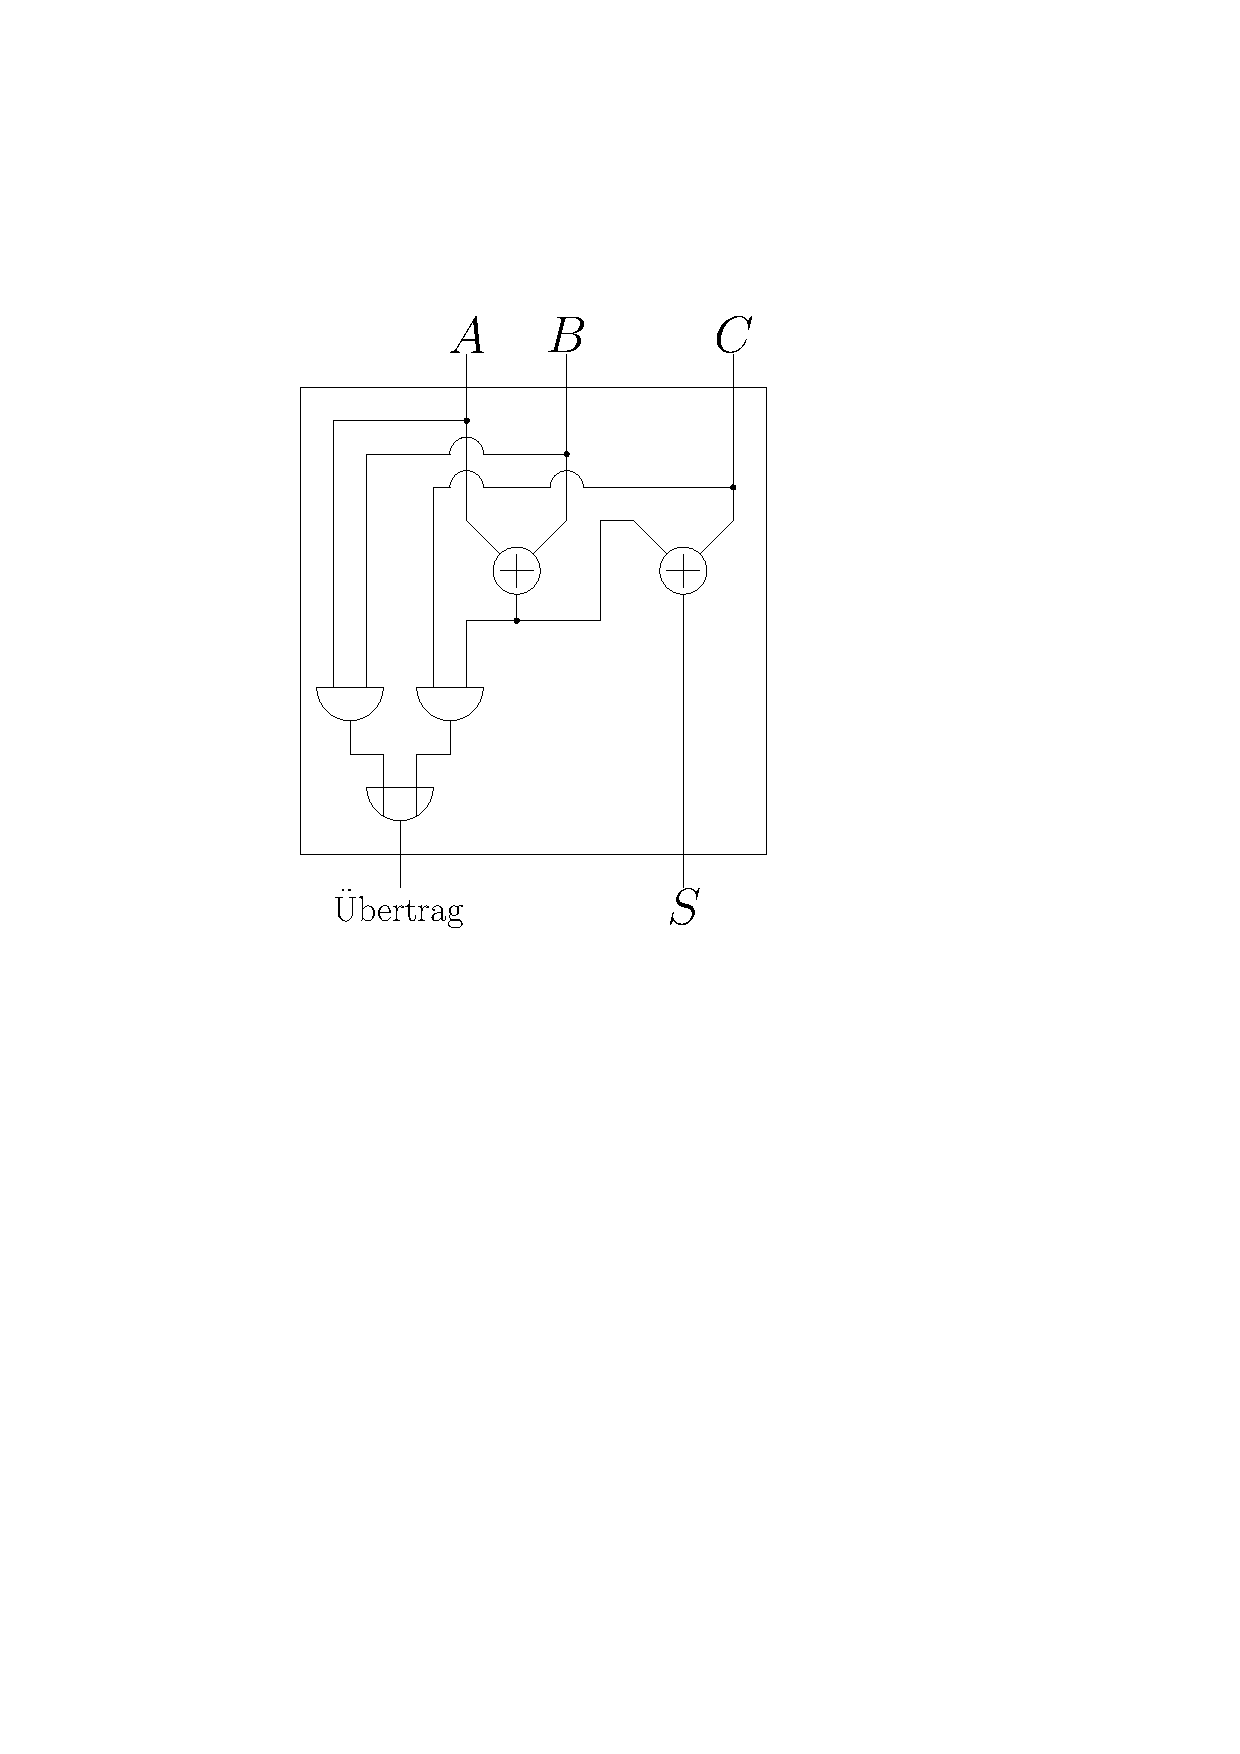
\includegraphics[scale=0.8]{bilder/Volladdierer_Detail.pdf}
\caption{Schaltkreis eines Volladdierers im Detail.}
\end{figure}

\noindent Die Tiefe eines Schaltkreises ist die maximale Zahl der Gatter auf einem Weg von einem Eingang zu einem Ausgang und entspricht der 
parallelen Laufzeit.
Die Gesamtzahl aller Gatter eines Schaltkreises nennt man seine Größe; sie entspricht dem Gesamtaufwand des Algorithmus.
\\
\\Aus $n$ Volladdierern kann man nun einen sogenannten Carry-Ripple-Adder zum Addieren zweier $n$-Bit-Zahlen 
zusammensetzen: 
\begin{figure}[h]
\centering
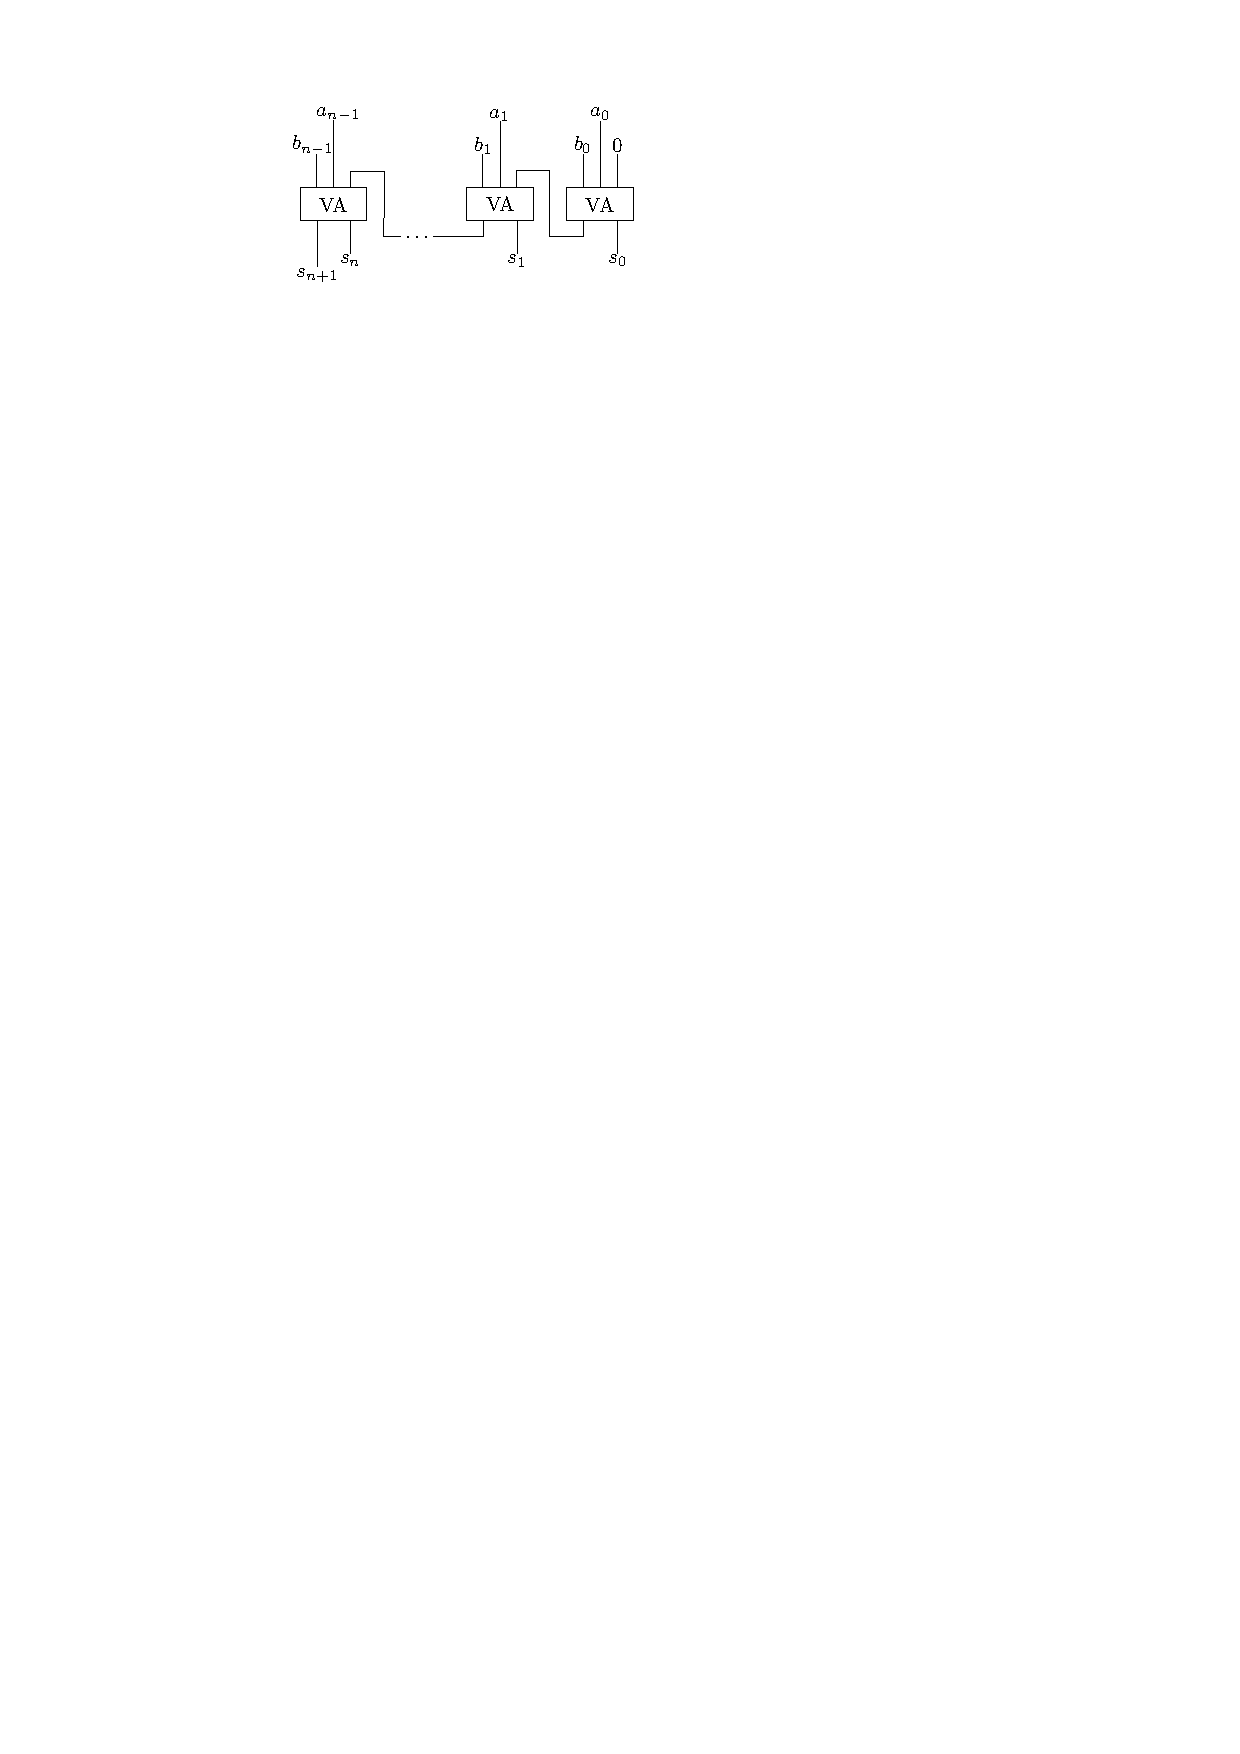
\includegraphics[scale=1.2]{bilder/Carry-Ripple-Adder.pdf}
\caption{Carry-Ripple-Adder.}
\end{figure}

\noindent Dessen Größe ist mit $O(n)$ gut, die Tiefe von $\theta(n)$ ist dagegen schlecht.
% \\{\bf{Frage}}: Geht es besser?
\\{\bf{Anmerkung:}}
\\Jeder $n$-Bit Addierer hat eine minimale Tiefe von $\Omega (\log n)$, da der Ausgang $s_{n+1}$ immer von allen Ausgängen abhängt, 
d.h. er muss mit allen verbunden sein. Wenn man alle Gatter betrachtet, die von $s_{n+1}$ aus erreichbar sind, ergibt sich
ein Binärbaum, da jedes Gatter maximal zwei Eingänge hat (evtl. Knoten mit nur einem). Die Blätter entsprechen den $2n$ Eingängen 
des Schaltkreises. Daraus ergibt sich eine minimale Höhe des Baumes von $\log (2n)$.
\\\\{\bf{Frage}}: Ist eine Tiefe $O(\log n)$ möglich? 
\\\\Ja, dies ist durch Vorausberechnung der Überträge möglich und kann mit dem soganannten ``Carry-Lookahead-Adder''
realisiert werden. Um diesen zu konstruieren, definieren wir den Schaltkreis $CLA_n$. 
F\"{u}hre dazu zun\"{a}chst eine neue Notation ein. 

Sei $n$ eine Zweierpotenz. Dann bezeichne $\bf{S_{i,l}}$ für $l=0,\dots,\log n$ und 
$i=0,\dots, \frac{n}{2^l}-1$ das Segment von $n-1, \dots, 0$, das von $(i+1)2^{l}-1$ bis $i2^{l}$ reicht:
\\\\
\begin{tabular}{|c|c|c|c|c|c|c|c|c|c|}
\hline  
$n-1$ & $n-2$ & $\dots$ & $(i+1)2^l-1$ & $\dots$ & $i2^l$ & $\dots$ & $2$ & $1$ & $0$ \\
\hline
\multicolumn{3}{|c|}{$\dots$}& \multicolumn{3}{c|}{ $S_{i,l}$ (i-tes Stück)} &  \multicolumn{4}{c|}{$\dots$}\\
\hline
\end{tabular}
\\
\\\\Der Schaltkreis $CLA_n$ berechnet zwei Bits, die wir wie folgt definieren:
\\$\bf{g_{i,l}} = 1$, wenn das Segment $S_{i,l}$ von $a$ und $b$ einen Übertrag ``erzeugt'' 
(wenn man beide addiert ohne die anderen Segmente zu betrachten)
\\$\bf{p_{i,l}} = 1$, wenn das Segement $S_{i,l}$ einen Übertrag propagiert, 
d.h., wenn von rechts ein Übertrag in das Segment hineinkommt, dann wird links auch einer weitergegeben.
\\Es gilt: 
\begin{eqnarray*}
g_{i,0} & = & a_i \wedge b_i \\
p_{i,0} & = & a_i \vee b_i \\
p_{i,l+1} & = &  p_{2i,l} \wedge p_{2i+1,l} \\
g_{i,l+1} & = & g_{2i+1,l} \vee (g_{2i,l} \wedge p_{2i+1,l})(i+1)2^{l+1}-1  
\end{eqnarray*}

\pagebreak
\noindent Der $CLA$ l\"{a}sst sich nun wie folgt rekursiv aufbauen:
\\\\Für $n = 1$:
\begin{figure}[h]
\centering
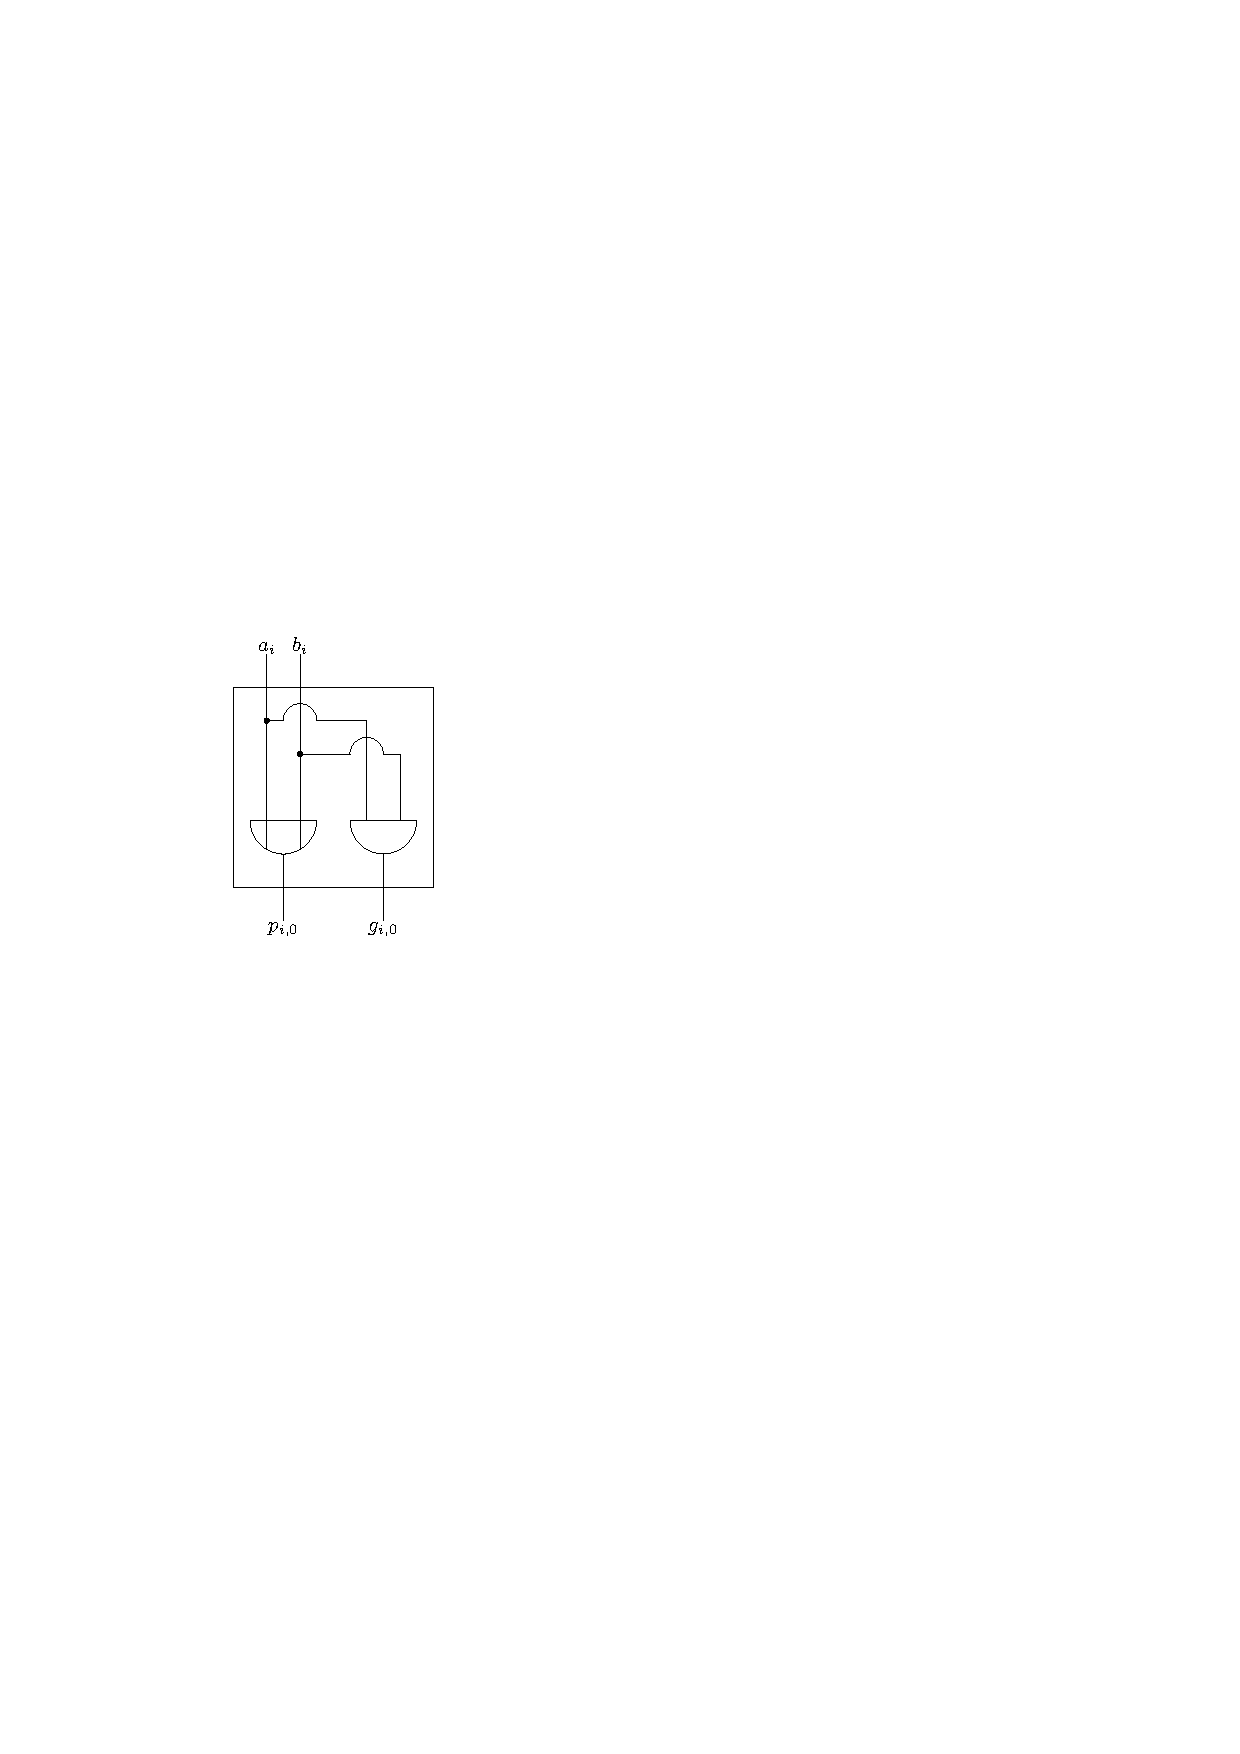
\includegraphics[scale=1.0]{bilder/CLA_1.pdf}
\caption{CLA für n=1.}
\end{figure}

Sonst ($n>1$): 
\begin{figure}[h!]
\centering
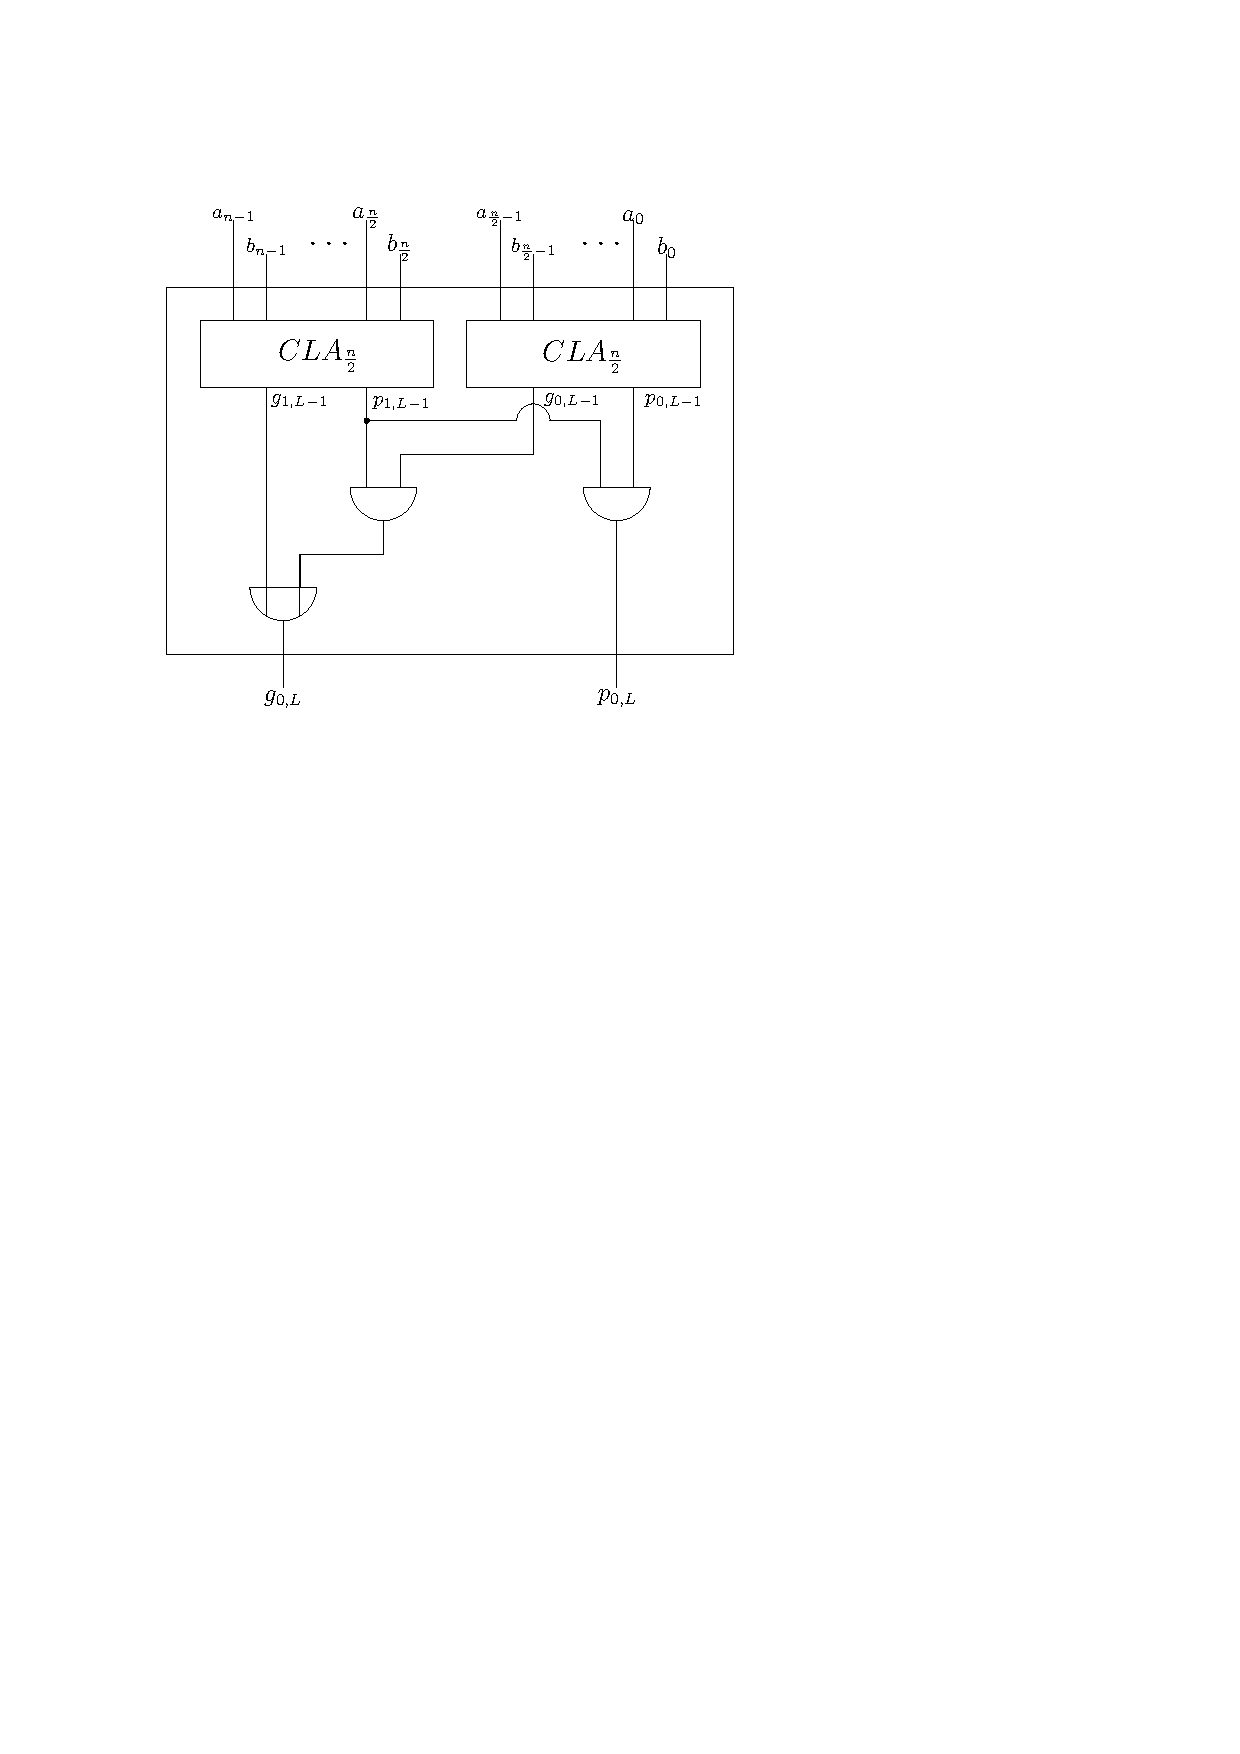
\includegraphics[scale=1.0]{bilder/CLA_n.pdf}
\caption{CLA für n=1.}
\end{figure}
\\Damit sind $p_{i,l}$ und $g_{i,l}$ für $l=0, \dots, L$ und 
$i=0, \dots, \frac{n}{2^l}-1$ in Tiefe $O(\log n)$ berechenbar.
\pagebreak
\\Mit Hilfe von $p_{i,l}$ und $g_{i,l}$ lassen sich nun die eigentlichen Überträge berechnen:
Sei $\bf{C_{i,l}}$ der Übertrag am Ende vom Segment $S_{i,l}$ (bei der Gesamtaddition). 
Dann gilt: 
\begin{eqnarray*}
c_{2i,l} & = & g_{2i,l} \vee (c_{i-1,l+1} \wedge p_{2i,l}) \\
c_{0,L} & = & g_{0,L} \\
c_{2i+1,l} & = & c_{i,l+1}
\end{eqnarray*}
